\subsection{Frontend}
\label{arquitecura:global_frontend}
Correspon a la part client del projecte, a través de la qual l'usuari final interactuarà amb el sistema (visualitzar pdf's, signar documents, etc.).\\
Com s'ha dit anteriorment, es pot interpretar el \textit{frontend} com una entitat independent, i com a entitat independent, disposa de la seva pròpia arquitectura, en aquest cas, arquitectura MVC\footnote{Model View Controller}.
\begin{figure}[h]
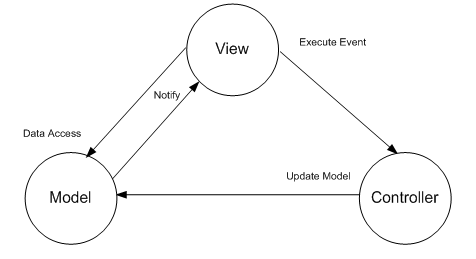
\includegraphics[scale=0.5]{sections/arquitectura/mvc.png}
\centering
\caption{Model-Vista-Controlador}
\label{fig:arquitectura_mvc}
\end{figure}
\newline L'arquitectura, ve donada pel mateix \textit{framework} que s'ha fet servir per al desenvolupament  (AngularJS).\\
\newline Per fer-ne un breu resum, aquesta arquitectura proposa distribuir els elements de codi en tres grups:
\begin{itemize}
    \item \textbf{Model}, representa les dades, s'encarrega de la seva gestió, rebre i servir. En aquest cas concret, s'encarrega de la comunicació amb el \textit{backend}, qui realment té les dades.
    \item \textbf{Vista}, el que veu l'usuari. Captura les interaccions i les transmet cap al controlador per que actui en conseqüència.
    \item \textbf{Controlador}, s'encarrega d'interpretar les interaccions que rep de la vista i modificar la vista en conseqüència.
\end{itemize}
Amb aquesta arquitectura, aconseguim un sistema modularitzat, amb dades sempre actualitzades i capes independents els uns dels altres.
\clearpage
 %donat que el client web no disposa d'\textit{storage} pròpi, entendrem com a model el component dins del projecte que s'encarrega de realitzar les peticions al \textbf{backend} i rebre'n els resultats (ja siguin satisfactoris o no).\\
\subsubsection{Diagrama de casos d'ús}
La tasca del \textit{frontend} és relativament senzilla.\\
Per una banda ha de permetre a l'usuari rebre la informació pertinent en cada cas i en cada moment. Per l'altra, ha de permetre a l'usuari ``jugar'' amb les dades i interactuar-hi.\\
Amb les anteriors premises, la component \textit{frontend} del projecte ha de ser capaç de permetre que l'usuari realitzi un seguit d'accions.\\
\newline La Figura \ref{fig:cas_us_frontend} mostra els casos d'ús (o accions) que necessàriament s'han de poder realitzar:
\begin{figure}[h]
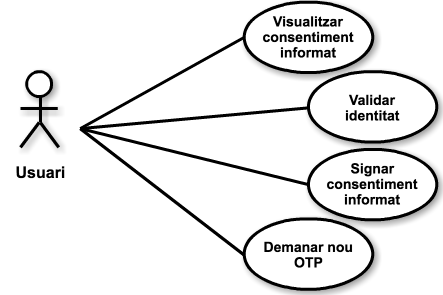
\includegraphics[scale=0.5]{sections/arquitectura/frontend_usecase.png}
\centering
\caption{Casos d'ús \textit{frontend}}
\label{fig:cas_us_frontend}
\end{figure}
\newline L'objectiu principal del \textit{frontend}, és permetre a l'usuari rebre les dades necessàries i donar el \textit{feedback} necessari per saber si l'operació de signatura s'ha dut a terme amb èxit o no.\\
\newline Així doncs, la part client del projecte té els següents propòsits:
\begin{itemize}
    \item Visualitzar consentiment informat:\\
    L'usuari ha de ser capaç de veure el consentiment informat dins de la mateixa plataforma. Alhora, hauria de ser capaç de descarregar-lo.
    \item Validació d'identitat:\\
    Abans de signar el document s'ha de validar la identitat del signant.
    \item Signatura consentiment informat:\\
    El sistema ha de permetre la signatura del document via OTP rebut per SMS.
    \item Demanar nou OTP:\\
    En cas de caducar el el codi enviat en el moment de la validació, l'usuari ha de ser capaç de demanar un nou codi OTP que li permeti signar el consentiment informat.
\end{itemize}
Aquestes quatre operacions, són les que el sistema d'emissió, validació i signatura electrònica de consentiment informats ha de tenir per a satisfer les necessitats bàsiques que es plantegen al projecte.\\
\newline Qualsevol afegit o bé característica addicional, ha de servir per complementar les anteriors.
%\clearpage
%Totes les operacions anteriors, es tradueixen en tot un seguit de crides HTTP a un backend mitjançant els mètodes GET i POST.

%Amb una cerca ràpida a \textit{Google} de la paraula \textit{frontend}, trobem la següent definició sota l'etiqueta \textit{computing}:
%\begin{displayquote}
%"\textit{\textbf{adj.} (of a device or program) directly accessed by the user and allowing access to further devices or programs.}"
%\end{displayquote}
%Tenint en compte l'anterior definició podem sobreentendre que la paraula \textit{frontend} fa referència a la part del projecte amb la que l'usuari interactuarà de forma directe, aquella que ha de permetre el visualitzar, signar i validar els consentiments informats que es generin amb la compra dels serveis a través de la plataforma; i fer-ho de la forma mes usable possible.\\
%\newline El \textit{frontend} s'ha desenvolupat amb \textit{AngularJS}\footnote{https://angularjs.org/}, un dels frameworks Javascript més estesos en el panorama \textit{web-development} actual.

%\subsection{AngularJS}
%\textit{AngularJS} és un framework per al desenvolupament d'aplicacions web dinàmiques, caracteritzat per ser de codi obert, basat en javascript i sobretot, mantingut principalment per \textit{Google} i una àmplia comunitat que s'esforça en donar solució als reptes que sorgeixen en el desenvolupament de les anomenades \textit{SPA} (\textit{Single Page Application}).\\
%\newline Un altre punt que ha posicionat fortament \textit{AngularJS} com un dels \textit{frameworks} per antonomàsia en el que fa a desenvolupament web, és l'us de l'arquitectura MVC (Model Vista Controlador), que ens permet distribuïr el codi i funcionalitats d'una forma coherent i fàcilment testejable.\\
%\newline Cap a finals de 2016 es va alliberar una versió estable del que s'anomena \textit{Angular2}, una revisió integral del framework web. Aquesta revisió suposa una reescriptura total del mateix, així com el canvi de funcionament de molts mòduls del propi \textit{framework}. Aquest pot ser un dels principals motius que l'adopció d'aquesta segona versió sigui lenta i costosa. \\
%\newline Actualment es consideren versions suportades les versions 2.4.1 i 1.6.1, sent aquesta última la més emprada sempre que es parla d'\textit{AngularJS}.\\
%\newline A grans trets, \textit{AngularJS} extén l'HTML aportant tot un seguit d'etiquetes, anomenades directives, que permeten als desenvolupadors coses com:
%\begin{itemize}
%    \item Control d'estructures del DOM
%    \item Amagar i mostrar elements del DOM
%    \item Validació dinàmica de formularis
%    \item Afegir nous comportaments a elements del DOM (gestió d'events...)
%    \item Reutilitzar HTML  agrupant-lo en components
%\end{itemize}
%\subsubsection{Single Page Application}
%El terme \textit{single page application} (SPA) es fa servir principalment amb aplicacions web que ofereixen un tipus d'interacció dinàmica i semblant al que trobariem en aplicacions mòbils o d'escriptori.\\
%\newline La principal diferècia entre una pàgina web corrent i una \textit{SPA}, és que aquesta última refresca molt poques vegades la pantalla. Una \textit{SPA} fa un ús intensiu d'AJAX, una forma de comunicar-se amb la part back-end servidora sense necessitat de refrescar la pàgina, que permet carregar les dades directament dins de la nostra aplicació, fent que aquestes es renderitzin directament sobre client.\\
%\newline En altres paraules, quan l'usuari accedeix per primera vegada a una \textit{SPA}, el navegador web descarregarà tota l'aplicació. Un cop descarregada, a mesura que l'usuari navegui, l'aplicació anirà descarregant la informació necessària i l'anirà pintant a mesura que faci falta i com faci falta. D'aquesta forma, s'aconsegueix una millor experiència d'usuari, ja que el que l'usuari final 
%\subsubsection{MVC}
%El patró anomenat model vista controlador (mvc) és un patró d'arquitectura del software que proposa el separar els components que formen el software en tres grans blocs. Per una banda el \textbf{model}, que correspon a tots els objectes de la lògica de negoci, també hi ha la \textbf{vista}, altrament dit interfície d'usuari o bé canal de comunicació amb altres programes, i finalment, el \textbf{controlador}, que gestiona tot el flux d'informació així com la comunicació entre el model i la vista.\\
%\newline Portat al context que ens ocupa, \textit{AngularJS}, es tradueix en tot un seguit de vistes, fitxers purament HTML, gestionades per controladors, fitxers Javascript, que vinculen dades i en controlen el comportament, i una bateria de serveis i llibreries, també fitxers Javascript, que són les encarregades de realitzar la comunicació amb el "món exterior".


